%%%%%%%%%%%%%%%%%%%%%%%%%%%%%%%%%%%%%%%%%
% Programming/Coding Assignment
% LaTeX Template
%
% This template has been downloaded from:
% http://www.latextemplates.com
%
% Original author:
% Ted Pavlic (http://www.tedpavlic.com)
%
% Note:
% The \lipsum[#] commands throughout this template generate dummy text
% to fill the template out. These commands should all be removed when 
% writing assignment content.
%
% This template uses a Perl script as an example snippet of code, most other
% languages are also usable. Configure them in the "CODE INCLUSION 
% CONFIGURATION" section.
%
%%%%%%%%%%%%%%%%%%%%%%%%%%%%%%%%%%%%%%%%%

%----------------------------------------------------------------------------------------
%	PACKAGES AND OTHER DOCUMENT CONFIGURATIONS
%----------------------------------------------------------------------------------------

%\documentclass{article}
\documentclass[12pt]{article}
\usepackage{fancyhdr} % Required for custom headers
\usepackage{lastpage} % Required to determine the last page for the footer
\usepackage{extramarks} % Required for headers and footers
\usepackage[usenames,dvipsnames]{color} % Required for custom colors
\usepackage{graphicx} % Required to insert images
\usepackage{subcaption}
\usepackage{listings} % Required for insertion of code
\usepackage{courier} % Required for the courier font
\usepackage{amsmath}
\usepackage{framed}

% Margins
\topmargin=-0.45in
\evensidemargin=0in
\oddsidemargin=0in
\textwidth=6.5in
\textheight=9.0in
\headsep=0.25in

\linespread{1.1} % Line spacing

% Set up the header and footer
\pagestyle{fancy}
\lhead{\hmwkAuthorName} % Top left header
\chead{\hmwkClass\ (\hmwkClassTime): \hmwkTitle} % Top center head
%\rhead{\firstxmark} % Top right header
\lfoot{\lastxmark} % Bottom left footer
\cfoot{} % Bottom center footer
\rfoot{Page\ \thepage\ of\ \protect\pageref{LastPage}} % Bottom right footer
\renewcommand\headrulewidth{0.4pt} % Size of the header rule
\renewcommand\footrulewidth{0.4pt} % Size of the footer rule

\setlength\parindent{0pt} % Removes all indentation from paragraphs

%----------------------------------------------------------------------------------------
%	CODE INCLUSION CONFIGURATION
%----------------------------------------------------------------------------------------

\definecolor{mygreen}{rgb}{0,0.6,0}
\definecolor{mygray}{rgb}{0.5,0.5,0.5}
\definecolor{mymauve}{rgb}{0.58,0,0.82}

\lstset{ %
  backgroundcolor=\color{white},   % choose the background color
  basicstyle=\footnotesize,        % size of fonts used for the code
  breaklines=true,                 % automatic line breaking only at whitespace
  captionpos=b,                    % sets the caption-position to bottom
  commentstyle=\color{mygreen},    % comment style
  escapeinside={\%*}{*)},          % if you want to add LaTeX within your code
  keywordstyle=\color{blue},       % keyword style
  stringstyle=\color{mymauve},     % string literal style
}

%----------------------------------------------------------------------------------------
%	DOCUMENT STRUCTURE COMMANDS
%	Skip this unless you know what you're doing
%----------------------------------------------------------------------------------------

% Header and footer for when a page split occurs within a problem environment
\newcommand{\enterProblemHeader}[1]{
%\nobreak\extramarks{#1}{#1 continued on next page\ldots}\nobreak
%\nobreak\extramarks{#1 (continued)}{#1 continued on next page\ldots}\nobreak
}

% Header and footer for when a page split occurs between problem environments
\newcommand{\exitProblemHeader}[1]{
%\nobreak\extramarks{#1 (continued)}{#1 continued on next page\ldots}\nobreak
%\nobreak\extramarks{#1}{}\nobreak
}

\setcounter{secnumdepth}{0} % Removes default section numbers
\newcounter{homeworkProblemCounter} % Creates a counter to keep track of the number of problems
\setcounter{homeworkProblemCounter}{0}

\newcommand{\homeworkProblemName}{}
\newenvironment{homeworkProblem}[1][Part \arabic{homeworkProblemCounter}]{ % Makes a new environment called homeworkProblem which takes 1 argument (custom name) but the default is "Problem #"
\stepcounter{homeworkProblemCounter} % Increase counter for number of problems
\renewcommand{\homeworkProblemName}{#1} % Assign \homeworkProblemName the name of the problem
\section{\homeworkProblemName} % Make a section in the document with the custom problem count
\enterProblemHeader{\homeworkProblemName} % Header and footer within the environment
}{
\exitProblemHeader{\homeworkProblemName} % Header and footer after the environment
}

\newcommand{\problemAnswer}[1]{ % Defines the problem answer command with the content as the only argument
\noindent\framebox[\columnwidth][c]{\begin{minipage}{0.98\columnwidth}#1\end{minipage}} % Makes the box around the problem answer and puts the content inside
}

\newcommand{\homeworkSectionName}{}
\newenvironment{homeworkSection}[1]{ % New environment for sections within homework problems, takes 1 argument - the name of the section
\renewcommand{\homeworkSectionName}{#1} % Assign \homeworkSectionName to the name of the section from the environment argument
\subsection{\homeworkSectionName} % Make a subsection with the custom name of the subsection
\enterProblemHeader{\homeworkProblemName\ [\homeworkSectionName]} % Header and footer within the environment
}{
\enterProblemHeader{\homeworkProblemName} % Header and footer after the environment
}

%----------------------------------------------------------------------------------------
%	NAME AND CLASS SECTION
%----------------------------------------------------------------------------------------

\newcommand{\hmwkTitle}{Programming Assignment 3} % Assignment title
\newcommand{\hmwkDueDate}{Thrusday, Mar 22, 2019} % Due date
\newcommand{\hmwkClass}{CSC421} % Course/class
\newcommand{\hmwkClassTime}{LEC 5101} % Class/lecture time
\newcommand{\hmwkAuthorName}{Zhongtian Ouyang} % Your name
\newcommand{\hmwkAuthorID}{1002341012} % Your ID


%----------------------------------------------------------------------------------------
%	TITLE PAGE
%----------------------------------------------------------------------------------------

\title{
\vspace{2in}
\textmd{\textbf{\hmwkClass:\ \hmwkTitle}}\\
\normalsize\vspace{0.1in}\small{Due\ on\ \hmwkDueDate}\\
\vspace{0.1in}
\vspace{3in}
}

\author{\textbf{\hmwkAuthorName}\\ \textbf{\hmwkAuthorID}}

\date{} % Insert date here if you want it to appear below your name

%----------------------------------------------------------------------------------------\
\begin{document}

\maketitle
\clearpage

%----------------------------------------------------------------------------------------
%	Common Tools
%----------------------------------------------------------------------------------------
%\begin{framed}
%\begin{lstlisting}[language=matlab]
%\end{lstlisting}
%\end{framed}

% \begin{bmatrix}
%0.5 & 0.6 \\ 
%0.7 & 0.8
%\end{bmatrix}

%\begin{figure}[h!]
%\centering
%\includegraphics[width=0.6\linewidth]{q10a.png}
%\label{fig:q10a}
%\end{figure}\\

%\begin{figure*}[!ht]
%\begin{subfigure}{.5\textwidth}
% \centering
%  \includegraphics[width=.5\linewidth]{p4_1.JPG}
%  \caption{Full set}
%  \label{fig:sfig1}
%\end{subfigure}
%\begin{subfigure}{.5\textwidth}
% \centering
%  \includegraphics[width=.5\linewidth]{P4_2.JPG}
%  \caption{Two each}
%  \label{fig:sfig2}
%\end{subfigure}%
%\caption{Part4 (a)}
%\label{fig:p4a}
%\end{figure*}

%\sum_{n=1}^{\infty} 2^{-n} = 1
%\prod_{i=a}^{b} f(i)
%----------------------------------------------------------------------------------------
%	PROBLEM 1
%----------------------------------------------------------------------------------------

% To have just one problem per page, simply put a \clearpage after each problem
\begin{homeworkProblem}
\noindent \textit{Encoder-Decoder Models and Teacher-Forcing}\\
1.\\
On long sequences, the architecture in Figure 1 will not perform well. The reason is that the architecture uses a fixed-length vector $h_T$ to represent the input sequence, and $h_T$ is the only information decoder can get. For a long sequence, $h_T$ won't be enough to represent all information of the input sequence. With a information loss, the decoder won't be able to make accurate character-wise predictions. Another reason is that the distance between the first input character and the first output character is too far away.\\

2.\\
(a) Increase the length of vector $h_T$ so that it is capable of storing information for long input sequence\\
(b) Reverse the input sequence.\\

3.\\
During training time, the input to the decoder at each time step is the ground-truth token. However, during testing time, the input will be the prediction in the previous time step. Therefore, if one of the predictions is incorrect, all the following predictions are very likely to be incorrect too since they were made based on incorrect inputs. The error accumulates. And the model won't be able to handle this problem because such problem doesn't exist during training.\\

4.\\ 
To address the issue with teacher forcing, we can accomodate the scheduled sampling proposed in the paper. Instead of always using ground-true token during training time, we would randomly choose to use the generated token or the ground-true token during training time. At the beginning, we will have a high probability for using ground-ture token and then gradually decrease such probably. At the end of training, we should mostly be using generated tokens.\\
\end{homeworkProblem}
\clearpage
%----------------------------------------------------------------------------------------
%	PROBLEM 2
%----------------------------------------------------------------------------------------

\begin{homeworkProblem}
\noindent \textit{Gated Recurrent Unit}\\
1.\\
In nmt.ipynb\\

2.\\
The result is not ideal, but OK. For the input ``the air conditioning is working'', the translated output is ``ehtay airway onitingsshay isway ouctingray''. We can see some of the words are correct: ``airway'', ``isway''. And for the incorrect words, the are somewhat resemble to the correct results: ``ehtay'' vs ``ethay''. Also, the model seems to understand the fact that a translated word always end with ``ay''. It seems like the model do better for shorter words as we would expect. \\

3.\\
The combination of ``th'' always become ``ht'' when moved to the back.\\
An incorrect character followed by more incorrect characters.\\
The first character moved to the back become something else incorrect.\\
Mess up the charcters in the middle for long words.\\
\end{homeworkProblem}
\clearpage
%----------------------------------------------------------------------------------------
%	PROBLEM 3
%----------------------------------------------------------------------------------------

\begin{homeworkProblem}
\noindent \textit{RNN with Attention}\\
1.\\
In nmt.ipynb\\

2.\\
In nmt.ipynb\\

3.\\
The results are overall better than the results from RNN decoder without attention. For shorter words, they are all correctly translated. For the longer words, many of them are correct; most of the incorrect ones only has a minor mistake. \\
Common Errors:\\
Missing letters in long words. Messing up at the end of a long word.\\
Training speed:\\
In terms of running time, to train for 100 epochs, the model with attention trains much slower, which is the same as the conclusion on the slides. The running time is longer because with attention, we need to calculate the attention context at each time step. Also, there are more weights to train for the model with attention.\\
In terms of epoch, the validation loss decrease faster for the model with attention.\\

4.\\
In nmt.ipynb\\
Compare to the additive attention, both the results and training speed are very similar. The reason is that when used within the RNN attention decoder, the function of the two attention method are very similar. The only differences are the function used to calculate f(Q, K), and the way context is calculated using attention and value.\\


\end{homeworkProblem}
\clearpage
%----------------------------------------------------------------------------------------
%	PROBLEM 4
%----------------------------------------------------------------------------------------

\begin{homeworkProblem}
\noindent \textit{Attention is All You Need}\\
1.\\
Additive attention:\\
Advantage:More flexible\\
Disadvantage:Needs two sequential steps because there are two layers and we need to calculate them one after another\\
Scaled dot-product attention:\\
Advantage:Can attend to multiple entries, more efficient due to matrix multiplication optimizations\\
Disadvantage:More parameters means slower to train and easier to overfit.\\

2.\\
In nmt.ipynb\\

3.\\
In nmt.ipynb\\
Compare to those from the previous decoders, the validation loss and training loss from transformer are much smaller. The actual translated texts are also better in quality. The sentence ``the air conditioning is working'' is correctly translated. And most of the words I tested are also correctly translated. \\
In terms of training speed, training transformer decoder for 100 epoches only takes about half of time compare to the previous decoders. Transformer decoder is faster to train as we expected.\\

4.\\
When training the model, we can observe that both losses are significantly higher. The results are very bad compare to the ones from causal model. Only very few words are correct, while the others are either blank or repetition of several letters. The reason is that without using causal attention for the self-attention, the model is trained to predict knowing both the previous and following characters. But when we test the decoder, it doesn't know the future. This discrepancy between training time and testing time make the decoder unable to perform well when making real predictions.\\

5.\\
Our simple transformer decoder work without explicit positional encoding because the sequence is relatively short in our model and the information about the positions of the input sequence is captured by the encoder annotations.

\end{homeworkProblem}
\clearpage
%----------------------------------------------------------------------------------------
%	PROBLEM 5
%----------------------------------------------------------------------------------------
\begin{homeworkProblem}
\noindent \textit{Attention Visualizations}\\

Word: cake $\rightarrow$ akecay\\
Correctly translated by both RNN and Transformer
\begin{figure}[h!]
\centering
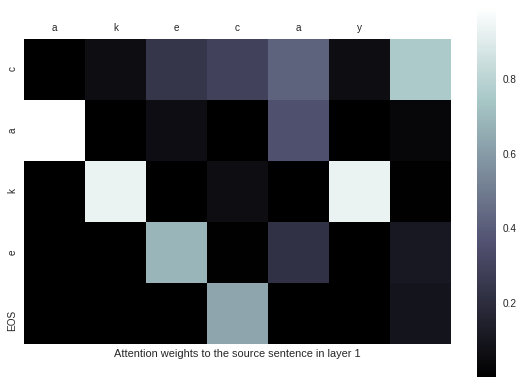
\includegraphics[width=0.5\linewidth]{cake-succ-rnn.png}
\caption{RNN Attention Map}
\label{fig:q10a}
\end{figure}
\begin{figure*}[!ht]
\begin{subfigure}{.3\textwidth}
 \centering
  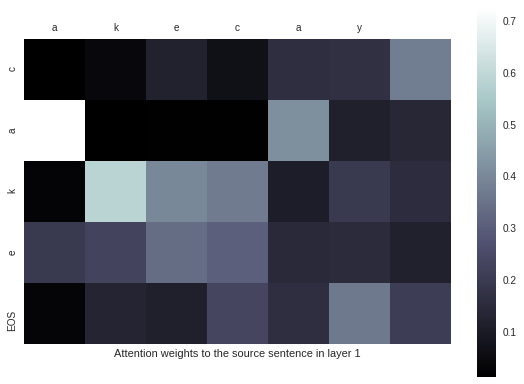
\includegraphics[width=\linewidth]{cake-succ-trans-1.png}
  \caption{layer 1}
\end{subfigure}
\begin{subfigure}{.3\textwidth}
 \centering
  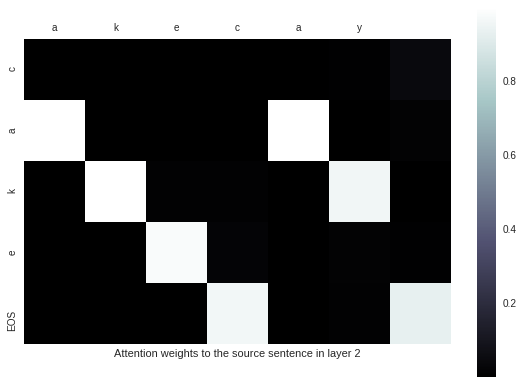
\includegraphics[width=\linewidth]{cake-succ-trans-2.png}
  \caption{layer 2}
\end{subfigure}
\begin{subfigure}{.3\textwidth}
 \centering
  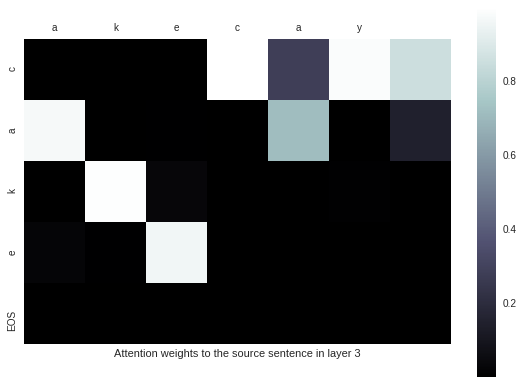
\includegraphics[width=\linewidth]{cake-succ-trans-3.png}
  \caption{layer 3}
\end{subfigure}
\caption{Transformer Attention Maps}
\end{figure*}

This is an example of a success case. We can see that in the rnn attention map , the attention for the characters ``a'', ``k'', ``e'' are almost perfect. The letter ``c'' has a somewhat split attention on ``c'' and EOS, which is reasonable because ``c'' should be at the position of EOS with the letter being ``c''. Attention for ``a'', ``y'' at the end of the word doesn't really matters because all the translated words should end with ``ay''.\\
For the transformer decoder, the attention in the first layer is rather scrambled. But in the layer, the attention is perfect. Notice that the attention for letter ``c'' in layer 2 and layer 3 indicates that the model understand that it should put an extra letter at EOS in this case and the letter should be the first letter.
\clearpage
Word: drink $\rightarrow$ inkdray\\
Correctly translated by both RNN and Transformer
\begin{figure}[h!]
\centering
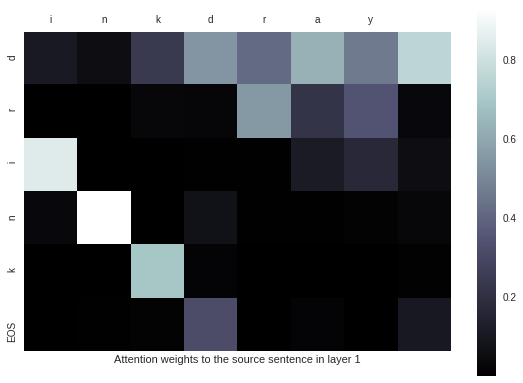
\includegraphics[width=0.5\linewidth]{drink-succ-rnn.png}
\caption{RNN Attention Map}
\label{fig:q10a}
\end{figure}
\begin{figure*}[!ht]
\begin{subfigure}{.3\textwidth}
 \centering
  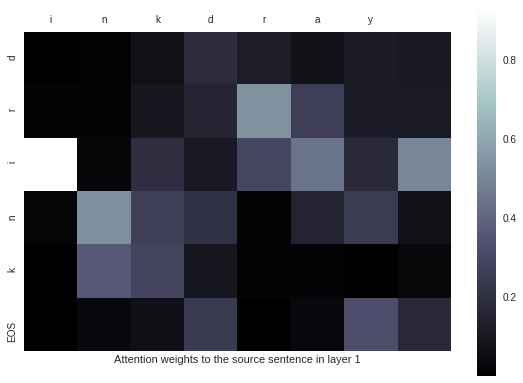
\includegraphics[width=\linewidth]{drink-succ-trans-1.png}
  \caption{layer 1}
\end{subfigure}
\begin{subfigure}{.3\textwidth}
 \centering
  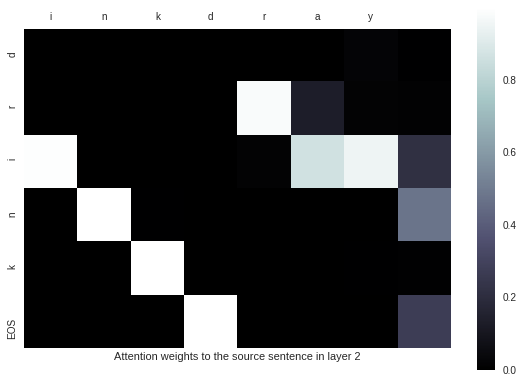
\includegraphics[width=\linewidth]{drink-succ-trans-2.png}
  \caption{layer 2}
\end{subfigure}
\begin{subfigure}{.3\textwidth}
 \centering
  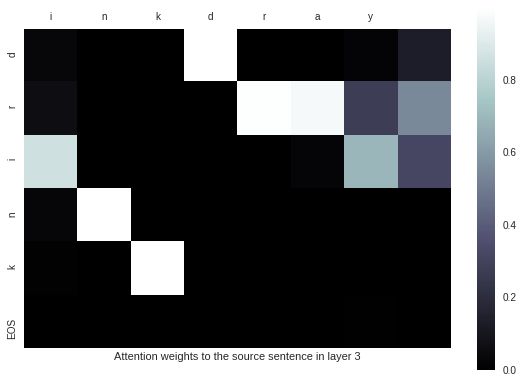
\includegraphics[width=\linewidth]{drink-succ-trans-3.png}
  \caption{layer 3}
\end{subfigure}
\caption{Transformer Attention Maps}
\end{figure*}

This is another success case. The Attention maps for both the RNN and Transformer are very similar to the previous case.

\clearpage
Word: aardvary $\rightarrow$ aardvaryway\\
Incorrectly translated by RNN. Correctly translated by Transformer\\
\begin{figure}[h!]
\centering
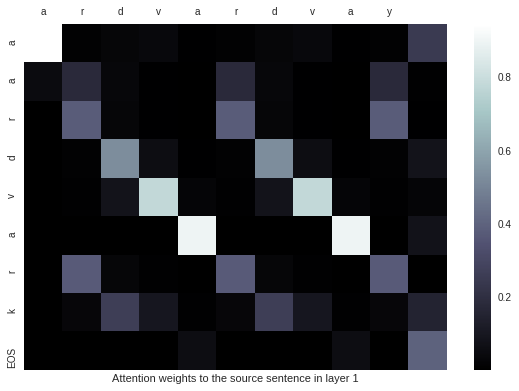
\includegraphics[width=0.5\linewidth]{aardvark-fail-rnn.png}
\caption{RNN Attention Map}
\label{fig:q10a}
\end{figure}
\begin{figure*}[!ht]
\begin{subfigure}{.3\textwidth}
 \centering
  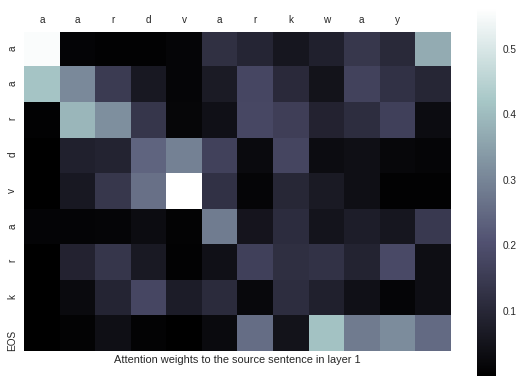
\includegraphics[width=\linewidth]{aardvark-succ-trans-1.png}
  \caption{layer 1}
\end{subfigure}
\begin{subfigure}{.3\textwidth}
 \centering
  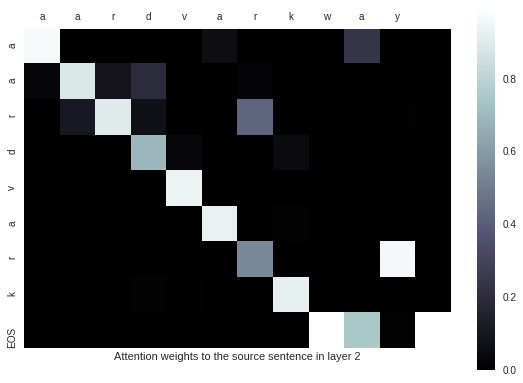
\includegraphics[width=\linewidth]{aardvark-succ-trans-2.png}
  \caption{layer 2}
\end{subfigure}
\begin{subfigure}{.3\textwidth}
 \centering
  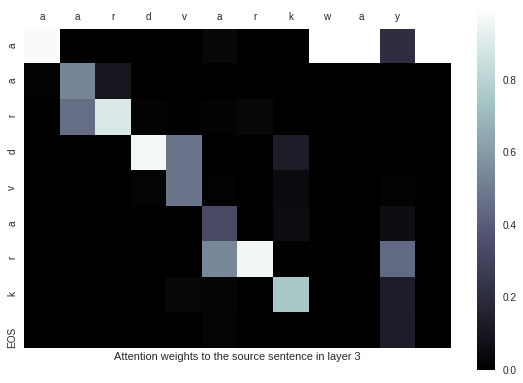
\includegraphics[width=\linewidth]{aardvark-succ-trans-3.png}
  \caption{layer 3}
\end{subfigure}
\caption{Transformer Attention Maps}
\end{figure*}

Here, the RNN fail to translate the word. Because of the unusual and repetitive structure the word has, the RNN is confused after the second ``a''. The attention is divided evenly between the two ``r'' characters, and mistakenly believe this character is the first ``r'' character instead, which resulted to a ``d'' instead of ``k'' and following errors.\\
As a comparison, we can see that the attention for the second and third layers of Transformer are concentrated on the diagonal. The letter ``w'' is also correctly added to the translated word by looking at the first letter and identifying it as a vowel.

\clearpage
Word: well-mannered $\rightarrow$ ellway-anneredmay\\
Correctly translated by RNN. Incorrectly translated by Transformer\\
\begin{figure}[h!]
\centering
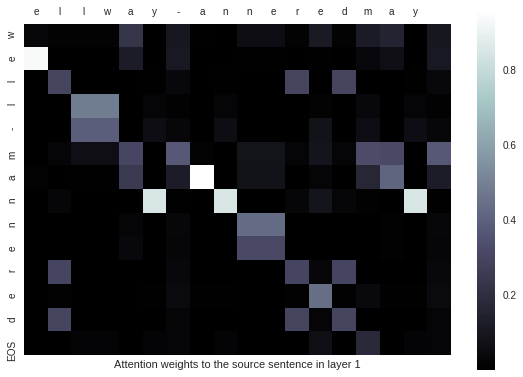
\includegraphics[width=0.5\linewidth]{well-mannered-succ-rnn.png}
\caption{RNN Attention Map}
\label{fig:q10a}
\end{figure}
\begin{figure*}[!ht]
\begin{subfigure}{.3\textwidth}
 \centering
  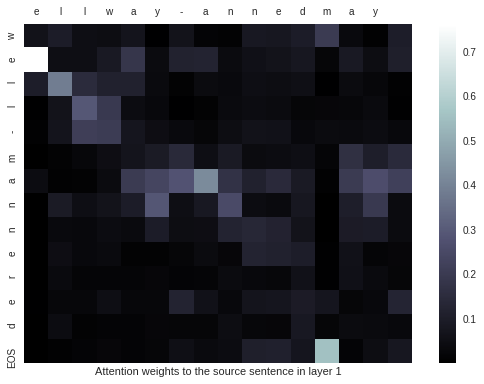
\includegraphics[width=\linewidth]{well-mannered-fail-trans-1.png}
  \caption{layer 1}
\end{subfigure}
\begin{subfigure}{.3\textwidth}
 \centering
  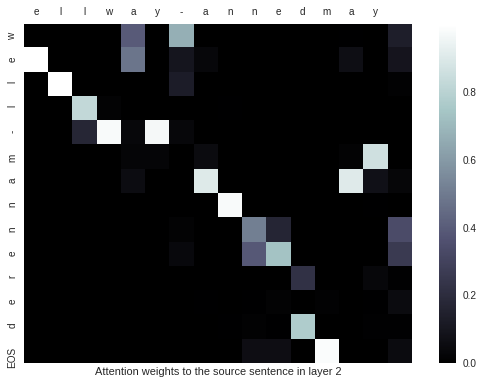
\includegraphics[width=\linewidth]{well-mannered-fail-trans-2.png}
  \caption{layer 2}
\end{subfigure}
\begin{subfigure}{.3\textwidth}
 \centering
  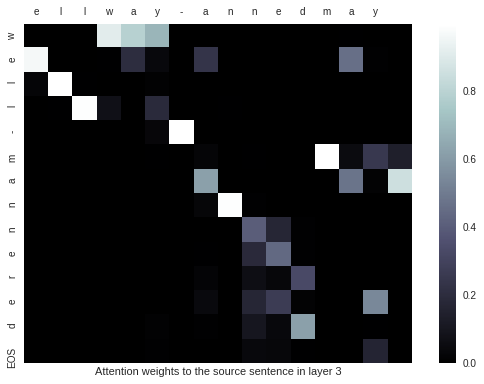
\includegraphics[width=\linewidth]{well-mannered-fail-trans-3.png}
  \caption{layer 3}
\end{subfigure}
\caption{Transformer Attention Maps}
\end{figure*}

Unexpectedly, in this case, RNN make the correct translation while Transformer doesn't. From RNN's attention map, we can see that the attention is in fact not very promising. The fact that it make a correct translation is accompanied with some luck. From Transformer's attention maps, we can see that it is confused after the first ``e'' in the word ``mannered''. It mistakenly attends to ``d'' after the second ``e'' instead of ``r'' which is the correct result.

\clearpage
Word: abcddcba $\rightarrow$ abcddcbaway\\
Incorrectly translated by RNN and Transformer\\
\begin{figure}[h!]
\centering
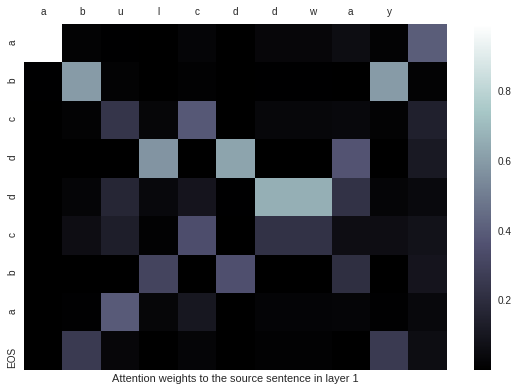
\includegraphics[width=0.5\linewidth]{abcddcba-fail-rnn.png}
\caption{RNN Attention Map}
\label{fig:q10a}
\end{figure}
\begin{figure*}[!ht]
\begin{subfigure}{.3\textwidth}
 \centering
  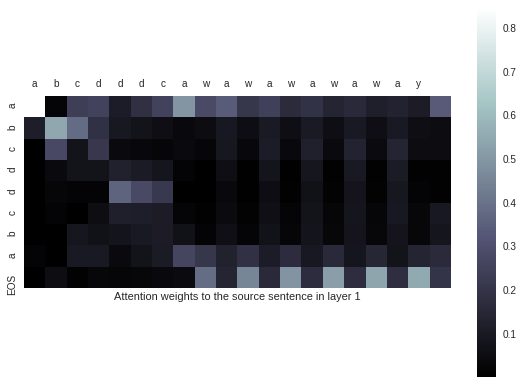
\includegraphics[width=\linewidth]{abcddcba-fail-trans-1.png}
  \caption{layer 1}
\end{subfigure}
\begin{subfigure}{.3\textwidth}
 \centering
  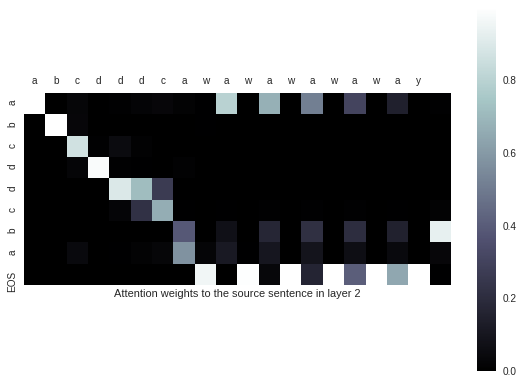
\includegraphics[width=\linewidth]{abcddcba-fail-trans-2.png}
  \caption{layer 2}
\end{subfigure}
\begin{subfigure}{.3\textwidth}
 \centering
  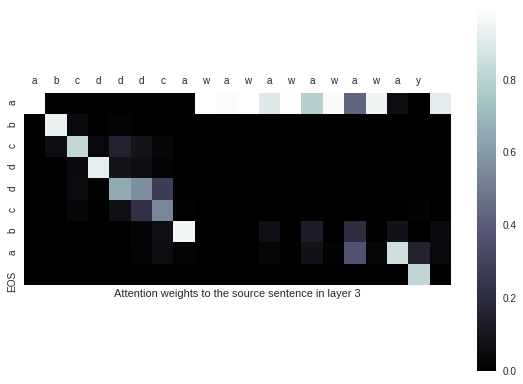
\includegraphics[width=\linewidth]{abcddcba-fail-trans-3.png}
  \caption{layer 3}
\end{subfigure}
\caption{Transformer Attention Maps}
\end{figure*}

Here, we can see the made-up word with unusual character combination and unusual symmetric structure gives both RNN and Transformer a hard time. For the RNN, we can observe that the top half and bottom half of the attention map is also somewhat symmetric. The symmetric structure makes RNN unable to attend to the correct letter and outputting random characters that was not exist in the original word. Transformer did a little bit better. The attention is mostly on the diagonal and the first part of the word is almost correct. However, Transformer seems to be unable to decide when to stop the word. The reason may be that the word is made up and the letter combinations are unusual.
\end{homeworkProblem}
\clearpage
%----------------------------------------------------------------------------------------

\end{document}
